
\begin{filecontents}{thesis.bib}
%http://en.wikibooks.org/wiki/LaTeX/Bibliography_Management

@inproceedings{podevijn2012self,
  title={Self-organised feedback in human swarm interaction},
  author={Podevijn, Ga{\"e}tan and O’Grady, Rehan and Dorigo, Marco},
  booktitle={Proceedings of the workshop on robot feedback in human-robot interaction: how to make a robot readable for a human interaction partner (Ro-Man 2012)},
  year={2012}
}

@incollection{podevijn2014gesturing,
  title={Gesturing at subswarms: Towards direct human control of robot swarms},
  author={Podevijn, Ga{\"e}tan and O’Grady, Rehan and Nashed, Youssef SG and Dorigo, Marco},
  booktitle={Towards Autonomous Robotic Systems},
  pages={390--403},
  year={2014},
  publisher={Springer}
}

@article{brambilla2013swarm,
  title={Swarm robotics: a review from the swarm engineering perspective},
  author={Brambilla, Manuele and Ferrante, Eliseo and Birattari, Mauro and Dorigo, Marco},
  journal={Swarm Intelligence},
  volume={7},
  number={1},
  pages={1--41},
  year={2013},
  publisher={Springer}
}

@incollection{csahin2005swarm,
  title={Swarm robotics: From sources of inspiration to domains of application},
  author={{\c{S}}ahin, Erol},
  booktitle={Swarm robotics},
  pages={10--20},
  year={2005},
  publisher={Springer}
}

@phdthesis{kazadi2000swarm,
  title={Swarm engineering},
  author={Kazadi, Sanza T},
  year={2000},
  school={California Institute of Technology}
}

@book{minsky1967computation,
  title={Computation: finite and infinite machines},
  author={Minsky, Marvin L},
  year={1967},
  publisher={Prentice-Hall, Inc.}
}

@article{granovetter1978threshold,
  title={Threshold models of collective behavior},
  author={Granovetter, Mark},
  journal={American journal of sociology},
  pages={1420--1443},
  year={1978},
  publisher={JSTOR}
}

@inproceedings{bonabeau1997adaptive,
  title={Adaptive Task Allocation Inspired by a Model of Division of Labor in Social Insects.},
  author={Bonabeau, Eric and Sobkowski, Andrej and Theraulaz, Guy and Deneubourg, Jean-Louis},
  booktitle={BCEC},
  pages={36--45},
  year={1997}
}

@article{bachrach2010composable,
  title={Composable continuous-space programs for robotic swarms},
  author={Bachrach, Jonathan and Beal, Jacob and McLurkin, James},
  journal={Neural Computing and Applications},
  volume={19},
  number={6},
  pages={825--847},
  year={2010},
  publisher={Springer}
}

@article{wolpert1999introduction,
  title={An introduction to collective intelligence},
  author={Wolpert, David H and Tumer, Kagan},
  journal={arXiv preprint cs/9908014},
  year={1999}
}

@article{abbott2006emergence,
  title={Emergence explained: Abstractions: Getting epiphenomena to do real work},
  author={Abbott, Russ},
  journal={Complexity},
  volume={12},
  number={1},
  pages={13--26},
  year={2006},
  publisher={Wiley Online Library}
}

@article{pinciroli2012argos,
  title={{ARGoS}: a Modular, Parallel, Multi-Engine Simulator for Multi-Robot Systems},
  author={Carlo Pinciroli and Vito Trianni and Rehan O'Grady and Giovanni Pini and Arne Brutschy and Manuele Brambilla and Nithin Mathews and Eliseo Ferrante and Gianni {Di Caro} and Frederick Ducatelle and Mauro Birattari and Luca Maria Gambardella and Marco Dorigo},
  journal={Swarm intelligence},
  volume={6},
  number={4},
  pages={271--295},
  year={2012},
  publisher={Springer},
  address = {Berlin, Germany},
  doi = {10.1007/s11721-012-0072-5}
}

@inproceedings{daily2003world,
  title={World embedded interfaces for human-robot interaction},
  author={Daily, Mike and Cho, Youngkwan and Martin, Kevin and Payton, Dave},
  booktitle={System Sciences, 2003. Proceedings of the 36th Annual Hawaii International Conference on},
  pages={6--pp},
  year={2003},
  organization={IEEE}
}

@incollection{baizid2009human,
  title={Human multi-robots interaction with high virtual reality abstraction level},
  author={Baizid, Khelifa and Li, Zhao and Mollet, Nicolas and Chellali, Ryad},
  booktitle={Intelligent Robotics and Applications},
  pages={23--32},
  year={2009},
  publisher={Springer}
}

@inproceedings{mclurkin2006speaking,
  title={Speaking Swarmish: Human-Robot Interface Design for Large Swarms of Autonomous Mobile Robots.},
  author={McLurkin, James and Smith, Jennifer and Frankel, James and Sotkowitz, David and Blau, David and Schmidt, Brian},
  booktitle={AAAI Spring Symposium: To Boldly Go Where No Human-Robot Team Has Gone Before},
  pages={72--75},
  year={2006}
}

@inproceedings{mondada2009puck,
  title={The e-puck, a robot designed for education in engineering},
  author={Mondada, Francesco and Bonani, Michael and Raemy, Xavier and Pugh, James and Cianci, Christopher and Klaptocz, Adam and Magnenat, Stephane and Zufferey, Jean-Christophe and Floreano, Dario and Martinoli, Alcherio},
  booktitle={Proceedings of the 9th conference on autonomous robot systems and competitions},
  volume={1},
  number={LIS-CONF-2009-004},
  pages={59--65},
  year={2009},
  organization={IPCB: Instituto Polit{\'e}cnico de Castelo Branco}
}

@misc{wiki:001,
   author = "Wikipedia",
   title = "Geta (footwear) --- Wikipedia{,} The Free Encyclopedia",
   year = "2015",
   url = "http://en.wikipedia.org/w/index.php?title=Geta_(footwear)&oldid=651925222",
   note = "[Online; accessed 20-May-2015]"
 }
 
 @misc{ wiki:002,
   author = "Wikipedia",
   title = "Walking --- Wikipedia{,} The Free Encyclopedia",
   year = "2015",
   url = "https://en.wikipedia.org/w/index.php?title=Walking&oldid=671922191",
   note = "[Online; accessed 1-August-2015]"
 }
 
 @misc{ wiki:003,
   author = "Wikipedia",
   title = "Box plot --- Wikipedia{,} The Free Encyclopedia",
   year = "2015",
   url = "https://en.wikipedia.org/w/index.php?title=Box_plot&oldid=669188116",
   note = "[Online; accessed 5-August-2015]"
 }
 
 @misc{ wiki:004,
   author = "Wikipedia",
   title = "ZCam --- Wikipedia{,} The Free Encyclopedia",
   year = "2014",
   url = "https://en.wikipedia.org/w/index.php?title=ZCam&oldid=639709035",
   note = "[Online; accessed 6-August-2015]"
 }
 
 @article{khatib1986real,
  title={Real-time obstacle avoidance for manipulators and mobile robots},
  author={Khatib, Oussama},
  journal={The international journal of robotics research},
  volume={5},
  number={1},
  pages={90--98},
  year={1986},
  publisher={Sage Publications}
}

@article{reif1999social,
  title={Social potential fields: A distributed behavioral control for autonomous robots},
  author={Reif, John H and Wang, Hongyan},
  journal={Robotics and Autonomous Systems},
  volume={27},
  number={3},
  pages={171--194},
  year={1999},
  publisher={Elsevier}
}

@article{spears2004distributed,
  title={Distributed, physics-based control of swarms of vehicles},
  author={Spears, William M and Spears, Diana F and Hamann, Jerry C and Heil, Rodney},
  journal={Autonomous Robots},
  volume={17},
  number={2-3},
  pages={137--162},
  year={2004},
  publisher={Springer}
}

@inproceedings{gutierrez2009open,
  title={Open e-puck range \& bearing miniaturized board for local communication in swarm robotics},
  author={Guti{\'e}rrez, {\'A}lvaro and Campo, Alexandre and Dorigo, Marco and Donate, Jesus and Monasterio-Huelin, F{\'e}lix and Magdalena, Luis},
  booktitle={Robotics and Automation, 2009. ICRA'09. IEEE International Conference on},
  pages={3111--3116},
  year={2009},
  organization={IEEE}
}

@techreport{stranieri2013iridia,
  author={A. Stranieri and A.E. Turgut and M. Salvaro and L. Garattoni and G. Francesca and A. Reina and M. Dorigo and  M. Birattari},
  title={IRIDIA's Arena Tracking System},
  institution={IRIDIA, Universit{\'e} Libre de Bruxelles},
  year={2013},
  number={TR/IRIDIA/2013-013},
  address={Brussels, Belgium},
  month={January}
}

@incollection{reinaaugmented,
  author = {Reina, Andreagiovanni and Salvaro, Mattia and Francesca, Gianpiero and Garattoni, Lorenzo and Pinciroli, Carlo and Dorigo, Marco and Birattari, Mauro},
  title = {Augmented reality for robots: virtual sensing technology applied to a swarm of e-pucks},
  booktitle = {2015 {NASA/ESA} Conference on Adaptive Hardware and Systems ({AHS 2015}))},
  publisher = {{IEEE} Computer Society Press},
  address = {Los Alamitos, CA},
  year = {2015},
  pages = {1--6},
  note = {Paper ID sB\_p3}
}

@techreport{GarFraBruPinBir2015:techreport-004,
 author={L. Garattoni and G. Francesca and A. Brutschy and C. Pinciroli and M. Birattari},
 title={Software Infrastructure for E-puck (and TAM)},
 institution={IRIDIA, Universit{\'e} Libre de Bruxelles},
 year={2015},
 number={TR/IRIDIA/2015-004},
 address={Brussels, Belgium},
 month={July}
}

@inproceedings{gritti2014kinect,
  title={Kinect-based people detection and tracking from small-footprint ground robots},
  author={Gritti, Armando Pesenti and Tarabini, Oscar and Guzzi, Jerome and Di Caro, Gianni and Caglioti, Vincenzo and Gambardella, Luca M and Giusti, Alessandro and others},
  booktitle={Intelligent Robots and Systems (IROS 2014), 2014 IEEE/RSJ International Conference on},
  pages={4096--4103},
  year={2014},
  organization={IEEE}
}

@misc{kinect,
	title={Microsoft Kinect},
	url={https://www.microsoft.com/en-us/kinectforwindows/},
	author={Microsoft},
	year={2015},
	note={Last consulted on 6th August 2015}
}

@misc{asus,
	title={Asus Xtion PRO LIVE},
	url={http://www.asus.com/be-fr/Multimedia/Xtion_PRO_LIVE/},
	author={Asus},
	year={2015},
	note={Last consulted on 6th August 2015}
}

@inproceedings{thrun1999minerva,
  title={MINERVA: A second-generation museum tour-guide robot},
  author={Thrun, Sebastian and Bennewitz, Maren and Burgard, Wolfram and Cremers, Armin B and Dellaert, Frank and Fox, Dieter and H{\"a}hnel, Dirk and Rosenberg, Charles and Roy, Nicholas and Schulte, Jamieson and others},
  booktitle={Robotics and automation, 1999. Proceedings. 1999 IEEE international conference on},
  volume={3},
  year={1999},
  organization={IEEE}
}

@inproceedings{reynolds1987flocks,
  title={Flocks, herds and schools: A distributed behavioral model},
  author={Reynolds, Craig W},
  booktitle={ACM Siggraph Computer Graphics},
  volume={21},
  number={4},
  pages={25--34},
  year={1987},
  organization={ACM}
}

@article{baldassarre2003evolving,
  title={Evolving mobile robots able to display collective behaviors},
  author={Baldassarre, Gianluca and Nolfi, Stefano and Parisi, Domenico},
  journal={Artificial life},
  volume={9},
  number={3},
  pages={255--267},
  year={2003},
  publisher={MIT Press}
}

@article{turgut2008self,
  title={Self-organized flocking in mobile robot swarms},
  author={Turgut, Ali E and {\c{C}}elikkanat, Hande and G{\"o}k{\c{c}}e, Fatih and {\c{S}}ahin, Erol},
  journal={Swarm Intelligence},
  volume={2},
  number={2-4},
  pages={97--120},
  year={2008},
  publisher={Springer}
}

@article{ccelikkanat2010steering,
  title={Steering self-organized robot flocks through externally guided individuals},
  author={{\c{C}}elikkanat, Hande and {\c{S}}ahin, Erol},
  journal={Neural Computing and Applications},
  volume={19},
  number={6},
  pages={849--865},
  year={2010},
  publisher={Springer}
}

@article{ferrante2012self,
  title={Self-organized flocking with a mobile robot swarm: a novel motion control method},
  author={Ferrante, Eliseo and Turgut, Ali Emre and Huepe, Cristi{\'a}n and Stranieri, Alessandro and Pinciroli, Carlo and Dorigo, Marco},
  journal={Adaptive Behavior},
  pages={1059712312462248},
  year={2012},
  publisher={SAGE Publications}
}

@article{dorigo2013swarmanoid,
  title={Swarmanoid: a novel concept for the study of heterogeneous robotic swarms},
  author={Dorigo, Marco and Floreano, Dario and Gambardella, Luca M and Mondada, Francesco and Nolfi, Stefano and Baaboura, Tarek and Birattari, Mauro and Bonani, Michael and Brambilla, Manuele and Brutschy, Arne and others},
  journal={Robotics \& Automation Magazine, IEEE},
  volume={20},
  number={4},
  pages={60--71},
  year={2013},
  publisher={IEEE}
}

@ARTICLE{Dorigo:2014,
AUTHOR = {Dorigo, M.  and Birattari, M.  and Brambilla, M. },
TITLE   = {{S}warm robotics},
YEAR	= 2014,
JOURNAL	= Scholarpedia,
VOLUME  = 9,
NUMBER  = 1,
PAGES   = 1463,
NOTE   = {{revision 138643}},
}

@misc{USNavy2014,
	title={U.S. Navy Tests Robot Boat Swarm to Overwhelm Enemies},
	url={http://spectrum.ieee.org/automaton/robotics/military-robots/us-navy-robot-boat-swarm},
	author={Jeremy Hsu},
	year={2014},
	note={Last consulted on 17th August 2015}
}

@inproceedings{bethel2009non,
  title={Non-facial and non-verbal affective expression in appearance-constrained robots for use in victim management: robots to the rescue!},
  author={Bethel, Cindy L and Bringes, Christine and Murphy, Robin R},
  booktitle={Proceedings of the 4th ACM/IEEE international conference on Human robot interaction},
  pages={191--192},
  year={2009},
  organization={ACM}
}

@inproceedings{dautenhahn2006may,
  title={How may I serve you?: a robot companion approaching a seated person in a helping context},
  author={Dautenhahn, Kerstin and Walters, M and Woods, Sarah and Koay, Kheng Lee and Nehaniv, Chrystopher L and Sisbot, A and Alami, Rachid and Sim{\'e}on, Thierry},
  booktitle={Proceedings of the 1st ACM SIGCHI/SIGART conference on Human-robot interaction},
  pages={172--179},
  year={2006},
  organization={ACM}
}

@inproceedings{itoh2006development,
  title={Development of a bioinstrumentation system in the interaction between a human and a robot},
  author={Itoh, Kazuko and Miwa, Hiroyasu and Nukariya, Yuko and Zecca, Massimiliano and Takanobu, Hideaki and Roccella, Stefano and Carrozza, Maria and Dario, Paolo and Takanishi, Atsuo},
  booktitle={Intelligent Robots and Systems, 2006 IEEE/RSJ International Conference on},
  pages={2620--2625},
  year={2006},
  organization={IEEE}
}

\end{filecontents}
%% bare_jrnl_compsoc.tex
%% V1.4a
%% 2014/09/17
%% by Michael Shell
%% See:
%% http://www.michaelshell.org/
%% for current contact information.
%%
%% This is a skeleton file demonstrating the use of IEEEtran.cls
%% (requires IEEEtran.cls version 1.8a or later) with an IEEE
%% Computer Society journal paper.
%%
%% Support sites:
%% http://www.michaelshell.org/tex/ieeetran/
%% http://www.ctan.org/tex-archive/macros/latex/contrib/IEEEtran/
%% and
%% http://www.ieee.org/

%%*************************************************************************
%% Legal Notice:
%% This code is offered as-is without any warranty either expressed or
%% implied; without even the implied warranty of MERCHANTABILITY or
%% FITNESS FOR A PARTICULAR PURPOSE! 
%% User assumes all risk.
%% In no event shall IEEE or any contributor to this code be liable for
%% any damages or losses, including, but not limited to, incidental,
%% consequential, or any other damages, resulting from the use or misuse
%% of any information contained here.
%%
%% All comments are the opinions of their respective authors and are not
%% necessarily endorsed by the IEEE.
%%
%% This work is distributed under the LaTeX Project Public License (LPPL)
%% ( http://www.latex-project.org/ ) version 1.3, and may be freely used,
%% distributed and modified. A copy of the LPPL, version 1.3, is included
%% in the base LaTeX documentation of all distributions of LaTeX released
%% 2003/12/01 or later.
%% Retain all contribution notices and credits.
%% ** Modified files should be clearly indicated as such, including  **
%% ** renaming them and changing author support contact information. **
%%
%% File list of work: IEEEtran.cls, IEEEtran_HOWTO.pdf, bare_adv.tex,
%%                    bare_conf.tex, bare_jrnl.tex, bare_conf_compsoc.tex,
%%                    bare_jrnl_compsoc.tex, bare_jrnl_transmag.tex
%%*************************************************************************


% *** Authors should verify (and, if needed, correct) their LaTeX system  ***
% *** with the testflow diagnostic prior to trusting their LaTeX platform ***
% *** with production work. IEEE's font choices and paper sizes can       ***
% *** trigger bugs that do not appear when using other class files.       ***                          ***
% The testflow support page is at:
% http://www.michaelshell.org/tex/testflow/


\documentclass[10pt,journal,compsoc]{IEEEtran}
%
% If IEEEtran.cls has not been installed into the LaTeX system files,
% manually specify the path to it like:
% \documentclass[10pt,journal,compsoc]{../sty/IEEEtran}





% Some very useful LaTeX packages include:
% (uncomment the ones you want to load)


% *** MISC UTILITY PACKAGES ***
%
%\usepackage{ifpdf}
% Heiko Oberdiek's ifpdf.sty is very useful if you need conditional
% compilation based on whether the output is pdf or dvi.
% usage:
% \ifpdf
%   % pdf code
% \else
%   % dvi code
% \fi
% The latest version of ifpdf.sty can be obtained from:
% http://www.ctan.org/tex-archive/macros/latex/contrib/oberdiek/
% Also, note that IEEEtran.cls V1.7 and later provides a builtin
% \ifCLASSINFOpdf conditional that works the same way.
% When switching from latex to pdflatex and vice-versa, the compiler may
% have to be run twice to clear warning/error messages.






% *** CITATION PACKAGES ***
%
\ifCLASSOPTIONcompsoc
  % IEEE Computer Society needs nocompress option
  % requires cite.sty v4.0 or later (November 2003)
  \usepackage[nocompress]{cite}
\else
  % normal IEEE
  \usepackage{cite}
\fi
% cite.sty was written by Donald Arseneau
% V1.6 and later of IEEEtran pre-defines the format of the cite.sty package
% \cite{} output to follow that of IEEE. Loading the cite package will
% result in citation numbers being automatically sorted and properly
% "compressed/ranged". e.g., [1], [9], [2], [7], [5], [6] without using
% cite.sty will become [1], [2], [5]--[7], [9] using cite.sty. cite.sty's
% \cite will automatically add leading space, if needed. Use cite.sty's
% noadjust option (cite.sty V3.8 and later) if you want to turn this off
% such as if a citation ever needs to be enclosed in parenthesis.
% cite.sty is already installed on most LaTeX systems. Be sure and use
% version 5.0 (2009-03-20) and later if using hyperref.sty.
% The latest version can be obtained at:
% http://www.ctan.org/tex-archive/macros/latex/contrib/cite/
% The documentation is contained in the cite.sty file itself.
%
% Note that some packages require special options to format as the Computer
% Society requires. In particular, Computer Society  papers do not use
% compressed citation ranges as is done in typical IEEE papers
% (e.g., [1]-[4]). Instead, they list every citation separately in order
% (e.g., [1], [2], [3], [4]). To get the latter we need to load the cite
% package with the nocompress option which is supported by cite.sty v4.0
% and later. Note also the use of a CLASSOPTION conditional provided by
% IEEEtran.cls V1.7 and later.





% *** GRAPHICS RELATED PACKAGES ***
%
\ifCLASSINFOpdf
  % \usepackage[pdftex]{graphicx}
  % declare the path(s) where your graphic files are
  % \graphicspath{{../pdf/}{../jpeg/}}
  % and their extensions so you won't have to specify these with
  % every instance of \includegraphics
  % \DeclareGraphicsExtensions{.pdf,.jpeg,.png}
\else
  % or other class option (dvipsone, dvipdf, if not using dvips). graphicx
  % will default to the driver specified in the system graphics.cfg if no
  % driver is specified.
  % \usepackage[dvips]{graphicx}
  % declare the path(s) where your graphic files are
  % \graphicspath{{../eps/}}
  % and their extensions so you won't have to specify these with
  % every instance of \includegraphics
  % \DeclareGraphicsExtensions{.eps}
\fi
% graphicx was written by David Carlisle and Sebastian Rahtz. It is
% required if you want graphics, photos, etc. graphicx.sty is already
% installed on most LaTeX systems. The latest version and documentation
% can be obtained at: 
% http://www.ctan.org/tex-archive/macros/latex/required/graphics/
% Another good source of documentation is "Using Imported Graphics in
% LaTeX2e" by Keith Reckdahl which can be found at:
% http://www.ctan.org/tex-archive/info/epslatex/
%
% latex, and pdflatex in dvi mode, support graphics in encapsulated
% postscript (.eps) format. pdflatex in pdf mode supports graphics
% in .pdf, .jpeg, .png and .mps (metapost) formats. Users should ensure
% that all non-photo figures use a vector format (.eps, .pdf, .mps) and
% not a bitmapped formats (.jpeg, .png). IEEE frowns on bitmapped formats
% which can result in "jaggedy"/blurry rendering of lines and letters as
% well as large increases in file sizes.
%
% You can find documentation about the pdfTeX application at:
% http://www.tug.org/applications/pdftex






% *** MATH PACKAGES ***
%
%\usepackage[cmex10]{amsmath}
% A popular package from the American Mathematical Society that provides
% many useful and powerful commands for dealing with mathematics. If using
% it, be sure to load this package with the cmex10 option to ensure that
% only type 1 fonts will utilized at all point sizes. Without this option,
% it is possible that some math symbols, particularly those within
% footnotes, will be rendered in bitmap form which will result in a
% document that can not be IEEE Xplore compliant!
%
% Also, note that the amsmath package sets \interdisplaylinepenalty to 10000
% thus preventing page breaks from occurring within multiline equations. Use:
%\interdisplaylinepenalty=2500
% after loading amsmath to restore such page breaks as IEEEtran.cls normally
% does. amsmath.sty is already installed on most LaTeX systems. The latest
% version and documentation can be obtained at:
% http://www.ctan.org/tex-archive/macros/latex/required/amslatex/math/





% *** SPECIALIZED LIST PACKAGES ***
%
%\usepackage{algorithmic}
% algorithmic.sty was written by Peter Williams and Rogerio Brito.
% This package provides an algorithmic environment fo describing algorithms.
% You can use the algorithmic environment in-text or within a figure
% environment to provide for a floating algorithm. Do NOT use the algorithm
% floating environment provided by algorithm.sty (by the same authors) or
% algorithm2e.sty (by Christophe Fiorio) as IEEE does not use dedicated
% algorithm float types and packages that provide these will not provide
% correct IEEE style captions. The latest version and documentation of
% algorithmic.sty can be obtained at:
% http://www.ctan.org/tex-archive/macros/latex/contrib/algorithms/
% There is also a support site at:
% http://algorithms.berlios.de/index.html
% Also of interest may be the (relatively newer and more customizable)
% algorithmicx.sty package by Szasz Janos:
% http://www.ctan.org/tex-archive/macros/latex/contrib/algorithmicx/




% *** ALIGNMENT PACKAGES ***
%
%\usepackage{array}
% Frank Mittelbach's and David Carlisle's array.sty patches and improves
% the standard LaTeX2e array and tabular environments to provide better
% appearance and additional user controls. As the default LaTeX2e table
% generation code is lacking to the point of almost being broken with
% respect to the quality of the end results, all users are strongly
% advised to use an enhanced (at the very least that provided by array.sty)
% set of table tools. array.sty is already installed on most systems. The
% latest version and documentation can be obtained at:
% http://www.ctan.org/tex-archive/macros/latex/required/tools/


% IEEEtran contains the IEEEeqnarray family of commands that can be used to
% generate multiline equations as well as matrices, tables, etc., of high
% quality.




% *** SUBFIGURE PACKAGES ***
%\ifCLASSOPTIONcompsoc
%  \usepackage[caption=false,font=footnotesize,labelfont=sf,textfont=sf]{subfig}
%\else
%  \usepackage[caption=false,font=footnotesize]{subfig}
%\fi
% subfig.sty, written by Steven Douglas Cochran, is the modern replacement
% for subfigure.sty, the latter of which is no longer maintained and is
% incompatible with some LaTeX packages including fixltx2e. However,
% subfig.sty requires and automatically loads Axel Sommerfeldt's caption.sty
% which will override IEEEtran.cls' handling of captions and this will result
% in non-IEEE style figure/table captions. To prevent this problem, be sure
% and invoke subfig.sty's "caption=false" package option (available since
% subfig.sty version 1.3, 2005/06/28) as this is will preserve IEEEtran.cls
% handling of captions.
% Note that the Computer Society format requires a sans serif font rather
% than the serif font used in traditional IEEE formatting and thus the need
% to invoke different subfig.sty package options depending on whether
% compsoc mode has been enabled.
%
% The latest version and documentation of subfig.sty can be obtained at:
% http://www.ctan.org/tex-archive/macros/latex/contrib/subfig/




% *** FLOAT PACKAGES ***
%
%\usepackage{fixltx2e}
% fixltx2e, the successor to the earlier fix2col.sty, was written by
% Frank Mittelbach and David Carlisle. This package corrects a few problems
% in the LaTeX2e kernel, the most notable of which is that in current
% LaTeX2e releases, the ordering of single and double column floats is not
% guaranteed to be preserved. Thus, an unpatched LaTeX2e can allow a
% single column figure to be placed prior to an earlier double column
% figure. The latest version and documentation can be found at:
% http://www.ctan.org/tex-archive/macros/latex/base/


%\usepackage{stfloats}
% stfloats.sty was written by Sigitas Tolusis. This package gives LaTeX2e
% the ability to do double column floats at the bottom of the page as well
% as the top. (e.g., "\begin{figure*}[!b]" is not normally possible in
% LaTeX2e). It also provides a command:
%\fnbelowfloat
% to enable the placement of footnotes below bottom floats (the standard
% LaTeX2e kernel puts them above bottom floats). This is an invasive package
% which rewrites many portions of the LaTeX2e float routines. It may not work
% with other packages that modify the LaTeX2e float routines. The latest
% version and documentation can be obtained at:
% http://www.ctan.org/tex-archive/macros/latex/contrib/sttools/
% Do not use the stfloats baselinefloat ability as IEEE does not allow
% \baselineskip to stretch. Authors submitting work to the IEEE should note
% that IEEE rarely uses double column equations and that authors should try
% to avoid such use. Do not be tempted to use the cuted.sty or midfloat.sty
% packages (also by Sigitas Tolusis) as IEEE does not format its papers in
% such ways.
% Do not attempt to use stfloats with fixltx2e as they are incompatible.
% Instead, use Morten Hogholm'a dblfloatfix which combines the features
% of both fixltx2e and stfloats:
%
% \usepackage{dblfloatfix}
% The latest version can be found at:
% http://www.ctan.org/tex-archive/macros/latex/contrib/dblfloatfix/




%\ifCLASSOPTIONcaptionsoff
%  \usepackage[nomarkers]{endfloat}
% \let\MYoriglatexcaption\caption
% \renewcommand{\caption}[2][\relax]{\MYoriglatexcaption[#2]{#2}}
%\fi
% endfloat.sty was written by James Darrell McCauley, Jeff Goldberg and 
% Axel Sommerfeldt. This package may be useful when used in conjunction with 
% IEEEtran.cls'  captionsoff option. Some IEEE journals/societies require that
% submissions have lists of figures/tables at the end of the paper and that
% figures/tables without any captions are placed on a page by themselves at
% the end of the document. If needed, the draftcls IEEEtran class option or
% \CLASSINPUTbaselinestretch interface can be used to increase the line
% spacing as well. Be sure and use the nomarkers option of endfloat to
% prevent endfloat from "marking" where the figures would have been placed
% in the text. The two hack lines of code above are a slight modification of
% that suggested by in the endfloat docs (section 8.4.1) to ensure that
% the full captions always appear in the list of figures/tables - even if
% the user used the short optional argument of \caption[]{}.
% IEEE papers do not typically make use of \caption[]'s optional argument,
% so this should not be an issue. A similar trick can be used to disable
% captions of packages such as subfig.sty that lack options to turn off
% the subcaptions:
% For subfig.sty:
% \let\MYorigsubfloat\subfloat
% \renewcommand{\subfloat}[2][\relax]{\MYorigsubfloat[]{#2}}
% However, the above trick will not work if both optional arguments of
% the \subfloat command are used. Furthermore, there needs to be a
% description of each subfigure *somewhere* and endfloat does not add
% subfigure captions to its list of figures. Thus, the best approach is to
% avoid the use of subfigure captions (many IEEE journals avoid them anyway)
% and instead reference/explain all the subfigures within the main caption.
% The latest version of endfloat.sty and its documentation can obtained at:
% http://www.ctan.org/tex-archive/macros/latex/contrib/endfloat/
%
% The IEEEtran \ifCLASSOPTIONcaptionsoff conditional can also be used
% later in the document, say, to conditionally put the References on a 
% page by themselves.




% *** PDF, URL AND HYPERLINK PACKAGES ***
%
%\usepackage{url}
% url.sty was written by Donald Arseneau. It provides better support for
% handling and breaking URLs. url.sty is already installed on most LaTeX
% systems. The latest version and documentation can be obtained at:
% http://www.ctan.org/tex-archive/macros/latex/contrib/url/
% Basically, \url{my_url_here}.





% *** Do not adjust lengths that control margins, column widths, etc. ***
% *** Do not use packages that alter fonts (such as pslatex).         ***
% There should be no need to do such things with IEEEtran.cls V1.6 and later.
% (Unless specifically asked to do so by the journal or conference you plan
% to submit to, of course. )


% correct bad hyphenation here
\hyphenation{op-tical net-works semi-conduc-tor}

\usepackage{hyperref}
\usepackage[pdftex]{graphicx}
\setlength\parskip{\baselineskip}

\begin{document}
%
% paper title
% Titles are generally capitalized except for words such as a, an, and, as,
% at, but, by, for, in, nor, of, on, or, the, to and up, which are usually
% not capitalized unless they are the first or last word of the title.
% Linebreaks \\ can be used within to get better formatting as desired.
% Do not put math or special symbols in the title.
\title{Human - Robots Swarms Interaction\\ \vspace{4mm} \Large{An Escorting Robot Swarm that Diverts a Human\\ away from Dangers one cannot perceive}}
%
%
% author names and IEEE memberships
% note positions of commas and nonbreaking spaces ( ~ ) LaTeX will not break
% a structure at a ~ so this keeps an author's name from being broken across
% two lines.
% use \thanks{} to gain access to the first footnote area
% a separate \thanks must be used for each paragraph as LaTeX2e's \thanks
% was not built to handle multiple paragraphs
%
%
%\IEEEcompsocitemizethanks is a special \thanks that produces the bulleted
% lists the Computer Society journals use for "first footnote" author
% affiliations. Use \IEEEcompsocthanksitem which works much like \item
% for each affiliation group. When not in compsoc mode,
% \IEEEcompsocitemizethanks becomes like \thanks and
% \IEEEcompsocthanksitem becomes a line break with idention. This
% facilitates dual compilation, although admittedly the differences in the
% desired content of \author between the different types of papers makes a
% one-size-fits-all approach a daunting prospect. For instance, compsoc 
% journal papers have the author affiliations above the "Manuscript
% received ..."  text while in non-compsoc journals this is reversed. Sigh.

\author{Anthony~Debruyn}% <-this % stops a space
%\IEEEcompsocitemizethanks{\IEEEcompsocthanksitem M. Shell is with the Department
%of Electrical and Computer Engineering, Georgia Institute of Technology, Atlanta,
%GA, 30332.\protect\\
%% note need leading \protect in front of \\ to get a newline within \thanks as
%% \\ is fragile and will error, could use \hfil\break instead.
%E-mail: see http://www.michaelshell.org/contact.html
%\IEEEcompsocthanksitem J. Doe and J. Doe are with Anonymous University.}% <-this % stops an unwanted space
%\thanks{Manuscript received April 19, 2005; revised September 17, 2014.}}

% note the % following the last \IEEEmembership and also \thanks - 
% these prevent an unwanted space from occurring between the last author name
% and the end of the author line. i.e., if you had this:
% 
% \author{....lastname \thanks{...} \thanks{...} }
%                     ^------------^------------^----Do not want these spaces!
%
% a space would be appended to the last name and could cause every name on that
% line to be shifted left slightly. This is one of those "LaTeX things". For
% instance, "\textbf{A} \textbf{B}" will typeset as "A B" not "AB". To get
% "AB" then you have to do: "\textbf{A}\textbf{B}"
% \thanks is no different in this regard, so shield the last } of each \thanks
% that ends a line with a % and do not let a space in before the next \thanks.
% Spaces after \IEEEmembership other than the last one are OK (and needed) as
% you are supposed to have spaces between the names. For what it is worth,
% this is a minor point as most people would not even notice if the said evil
% space somehow managed to creep in.



% The paper headers
\markboth{Universit\'{e} Libre de Bruxelles, \'{E}cole Polytechnique de Bruxelles}%
{Shell \MakeLowercase{\textit{et al.}}: Bare Demo of IEEEtran.cls for Computer Society Journals}
% The only time the second header will appear is for the odd numbered pages
% after the title page when using the twoside option.
% 
% *** Note that you probably will NOT want to include the author's ***
% *** name in the headers of peer review papers.                   ***
% You can use \ifCLASSOPTIONpeerreview for conditional compilation here if
% you desire.



% The publisher's ID mark at the bottom of the page is less important with
% Computer Society journal papers as those publications place the marks
% outside of the main text columns and, therefore, unlike regular IEEE
% journals, the available text space is not reduced by their presence.
% If you want to put a publisher's ID mark on the page you can do it like
% this:
%\IEEEpubid{0000--0000/00\$00.00~\copyright~2014 IEEE}
% or like this to get the Computer Society new two part style.
%\IEEEpubid{\makebox[\columnwidth]{\hfill 0000--0000/00/\$00.00~\copyright~2014 IEEE}%
%\hspace{\columnsep}\makebox[\columnwidth]{Published by the IEEE Computer Society\hfill}}
% Remember, if you use this you must call \IEEEpubidadjcol in the second
% column for its text to clear the IEEEpubid mark (Computer Society jorunal
% papers don't need this extra clearance.)



% use for special paper notices
%\IEEEspecialpapernotice{(Invited Paper)}



% for Computer Society papers, we must declare the abstract and index terms
% PRIOR to the title within the \IEEEtitleabstractindextext IEEEtran
% command as these need to go into the title area created by \maketitle.
% As a general rule, do not put math, special symbols or citations
% in the abstract or keywords.
\IEEEtitleabstractindextext{%
%\begin{abstract}
%The abstract goes here.
%\end{abstract}
%
%% Note that keywords are not normally used for peerreview papers.
%\begin{IEEEkeywords}
%Computer Society, IEEEtran, journal, \LaTeX, paper, template.
%\end{IEEEkeywords}
\center August 17, 2015
}


% make the title area
\maketitle


% To allow for easy dual compilation without having to reenter the
% abstract/keywords data, the \IEEEtitleabstractindextext text will
% not be used in maketitle, but will appear (i.e., to be "transported")
% here as \IEEEdisplaynontitleabstractindextext when the compsoc 
% or transmag modes are not selected <OR> if conference mode is selected 
% - because all conference papers position the abstract like regular
% papers do.
\IEEEdisplaynontitleabstractindextext
% \IEEEdisplaynontitleabstractindextext has no effect when using
% compsoc or transmag under a non-conference mode.



% For peer review papers, you can put extra information on the cover
% page as needed:
% \ifCLASSOPTIONpeerreview
% \begin{center} \bfseries EDICS Category: 3-BBND \end{center}
% \fi
%
% For peerreview papers, this IEEEtran command inserts a page break and
% creates the second title. It will be ignored for other modes.
\IEEEpeerreviewmaketitle



%\IEEEraisesectionheading{\section{Introduction}\label{sec:introduction}}
% Computer Society journal (but not conference!) papers do something unusual
% with the very first section heading (almost always called "Introduction").
% They place it ABOVE the main text! IEEEtran.cls does not automatically do
% this for you, but you can achieve this effect with the provided
% \IEEEraisesectionheading{} command. Note the need to keep any \label that
% is to refer to the section immediately after \section in the above as
% \IEEEraisesectionheading puts \section within a raised box.




% The very first letter is a 2 line initial drop letter followed
% by the rest of the first word in caps (small caps for compsoc).
% 
% form to use if the first word consists of a single letter:
% \IEEEPARstart{A}{demo} file is ....
% 
% form to use if you need the single drop letter followed by
% normal text (unknown if ever used by IEEE):
% \IEEEPARstart{A}{}demo file is ....
% 
% Some journals put the first two words in caps:
% \IEEEPARstart{T}{his demo} file is ....
% 
% Here we have the typical use of a "T" for an initial drop letter
% and "HIS" in caps to complete the first word.
\IEEEPARstart{N}{ew} progresses in robotics have opened a new branch of studies. Taking inspiration from social animals like ants, bees or fishes, researchers are now able to create groups of robots performing tasks that could not be undertaken individually. These groups are called swarms. We envision swarm robotics to be useful for applications like search and rescue, environment exploration, or oil spill cleaning \cite{Dorigo:2014}. In swarm robotics system, each robot executes the same controller code. The interaction between the robots and between the robots and the environment enable the emergence of a collective behaviour. There is no hierarchy in the swarm. That is, all the robots behave autonomously. Research in swarm robotics is important as it underpins potential future disruptive innovations. Nanorobotics is going to be one of these innovations. The use of nanorobotics in medicine will grow over the next years. It could be one of the future solutions to cure cancer or other diseases by targeting the faulty constituents of the body with a swarm of very small robots. Swarm robotics is also important because it could constitute an adequate solution to other real problems. Swarm robotics systems are robust, i.e., losing a robot of the swarm is not a critical issue. Some tasks are dangerous for humans (e.g., demining, search and rescue) and the use of robots is preferred to avoid any injuries. However there is also a high risk of losing robots. Hence this task requires a fault-tolerant approach that swarm robotics can provide. Thanks to their scalability and flexibility, swarm robotics solutions are also suitable for applications where it is difficult to estimate the resources needed to carry out the task (e.g., search and rescue, cleaning). Swarm robotics solutions quickly adapt to new operation conditions and are thus appropriate for tasks in environments that change over time (e.g., patrolling, disaster recovery, and search and rescue). Since the robots behave autonomously, swarm robotics solutions are also suitable for large or unstructured environments where no infrastructure, like a communication system or a global localisation system, can be used to control the robots. Examples are underwater or extra-terrestrial planetary exploration, surveillance, demining, and search and rescue \cite{Dorigo:2014}.

Even though swarm robotics can carry out tasks autonomously, they do not have a global understanding of the environment and of the task that they must carry out. A human operator can, therefore, interact with those swarm systems to issue them commands (i.e., what type of tasks to carry out and where to carry out the task). Issuing commands relies on a one-way communication between the human and the swarm of robots. For swarm robotics to be adopted outside of research laboratories and tackle real world issues, one should always be able to take control of the swarm at any time. This is a legitimate safety requirement when considering the use of a large amount of potentially harmful robots around humans. Hence one can understand the vital aspect of the interaction between human and swarms of robots. In this thesis, however, we did not implement a method granting the human to completely control the swarm. We leave it as a future work. For the purpose of this thesis, it was not necessary.

To date, little attention has been paid to robotics swarm feedback, i.e., messages sent from the swarm to the human operator. Most of the research works focus on issuing commands to swarms. However, there might be situations in which the human does not know everything (e.g., where a gas leak comes from). For instance, we can leverage swarm robotics systems to help humans move in dangerous environments. To the best of our knowledge, no study has considered a human being escorted by a swarm of robots in a dangerous environment.

In this thesis we make an attempt to address this lack of consideration. We study how a swarm of robots can help a human move in dangerous environments. We use inspiration from flocking and pattern formation to allow a swarm of robots (see Figure \ref{fig:e-puck}) to prevent a human from entering dangerous areas. In this thesis, these dangerous areas are invisible to the human. These dangerous areas could, for instance, contain mines or be radioactive, or present another type of danger (e.g., poisonous gas, unstable floor). In order for the human to avoid these dangerous areas, we designed a swarm system that escorts the human in an environment. The robots encircle the human. There is a bidirectional feedback between the swarm and the human. The robots warn the human about the danger, and the human indirectly controls the position of the robots by changing his/her position. The swarm is augmenting the capabilities of the human. The human is able to perceive dangers that he would not be able to perceive without the help of our robotic system. It contrasts with most of the studies that only contain a unidirectional feedback (the human controlling the swarm). For the robots to stay around the human, we had to find a way to make the human detectable for the robots. We built an entirely new portable device for that purpose: augmented shoes with coloured LEDs that the robots can detect with their camera (see Figure \ref{fig:shoes}).

\begin{figure}[!t]
	\centering
	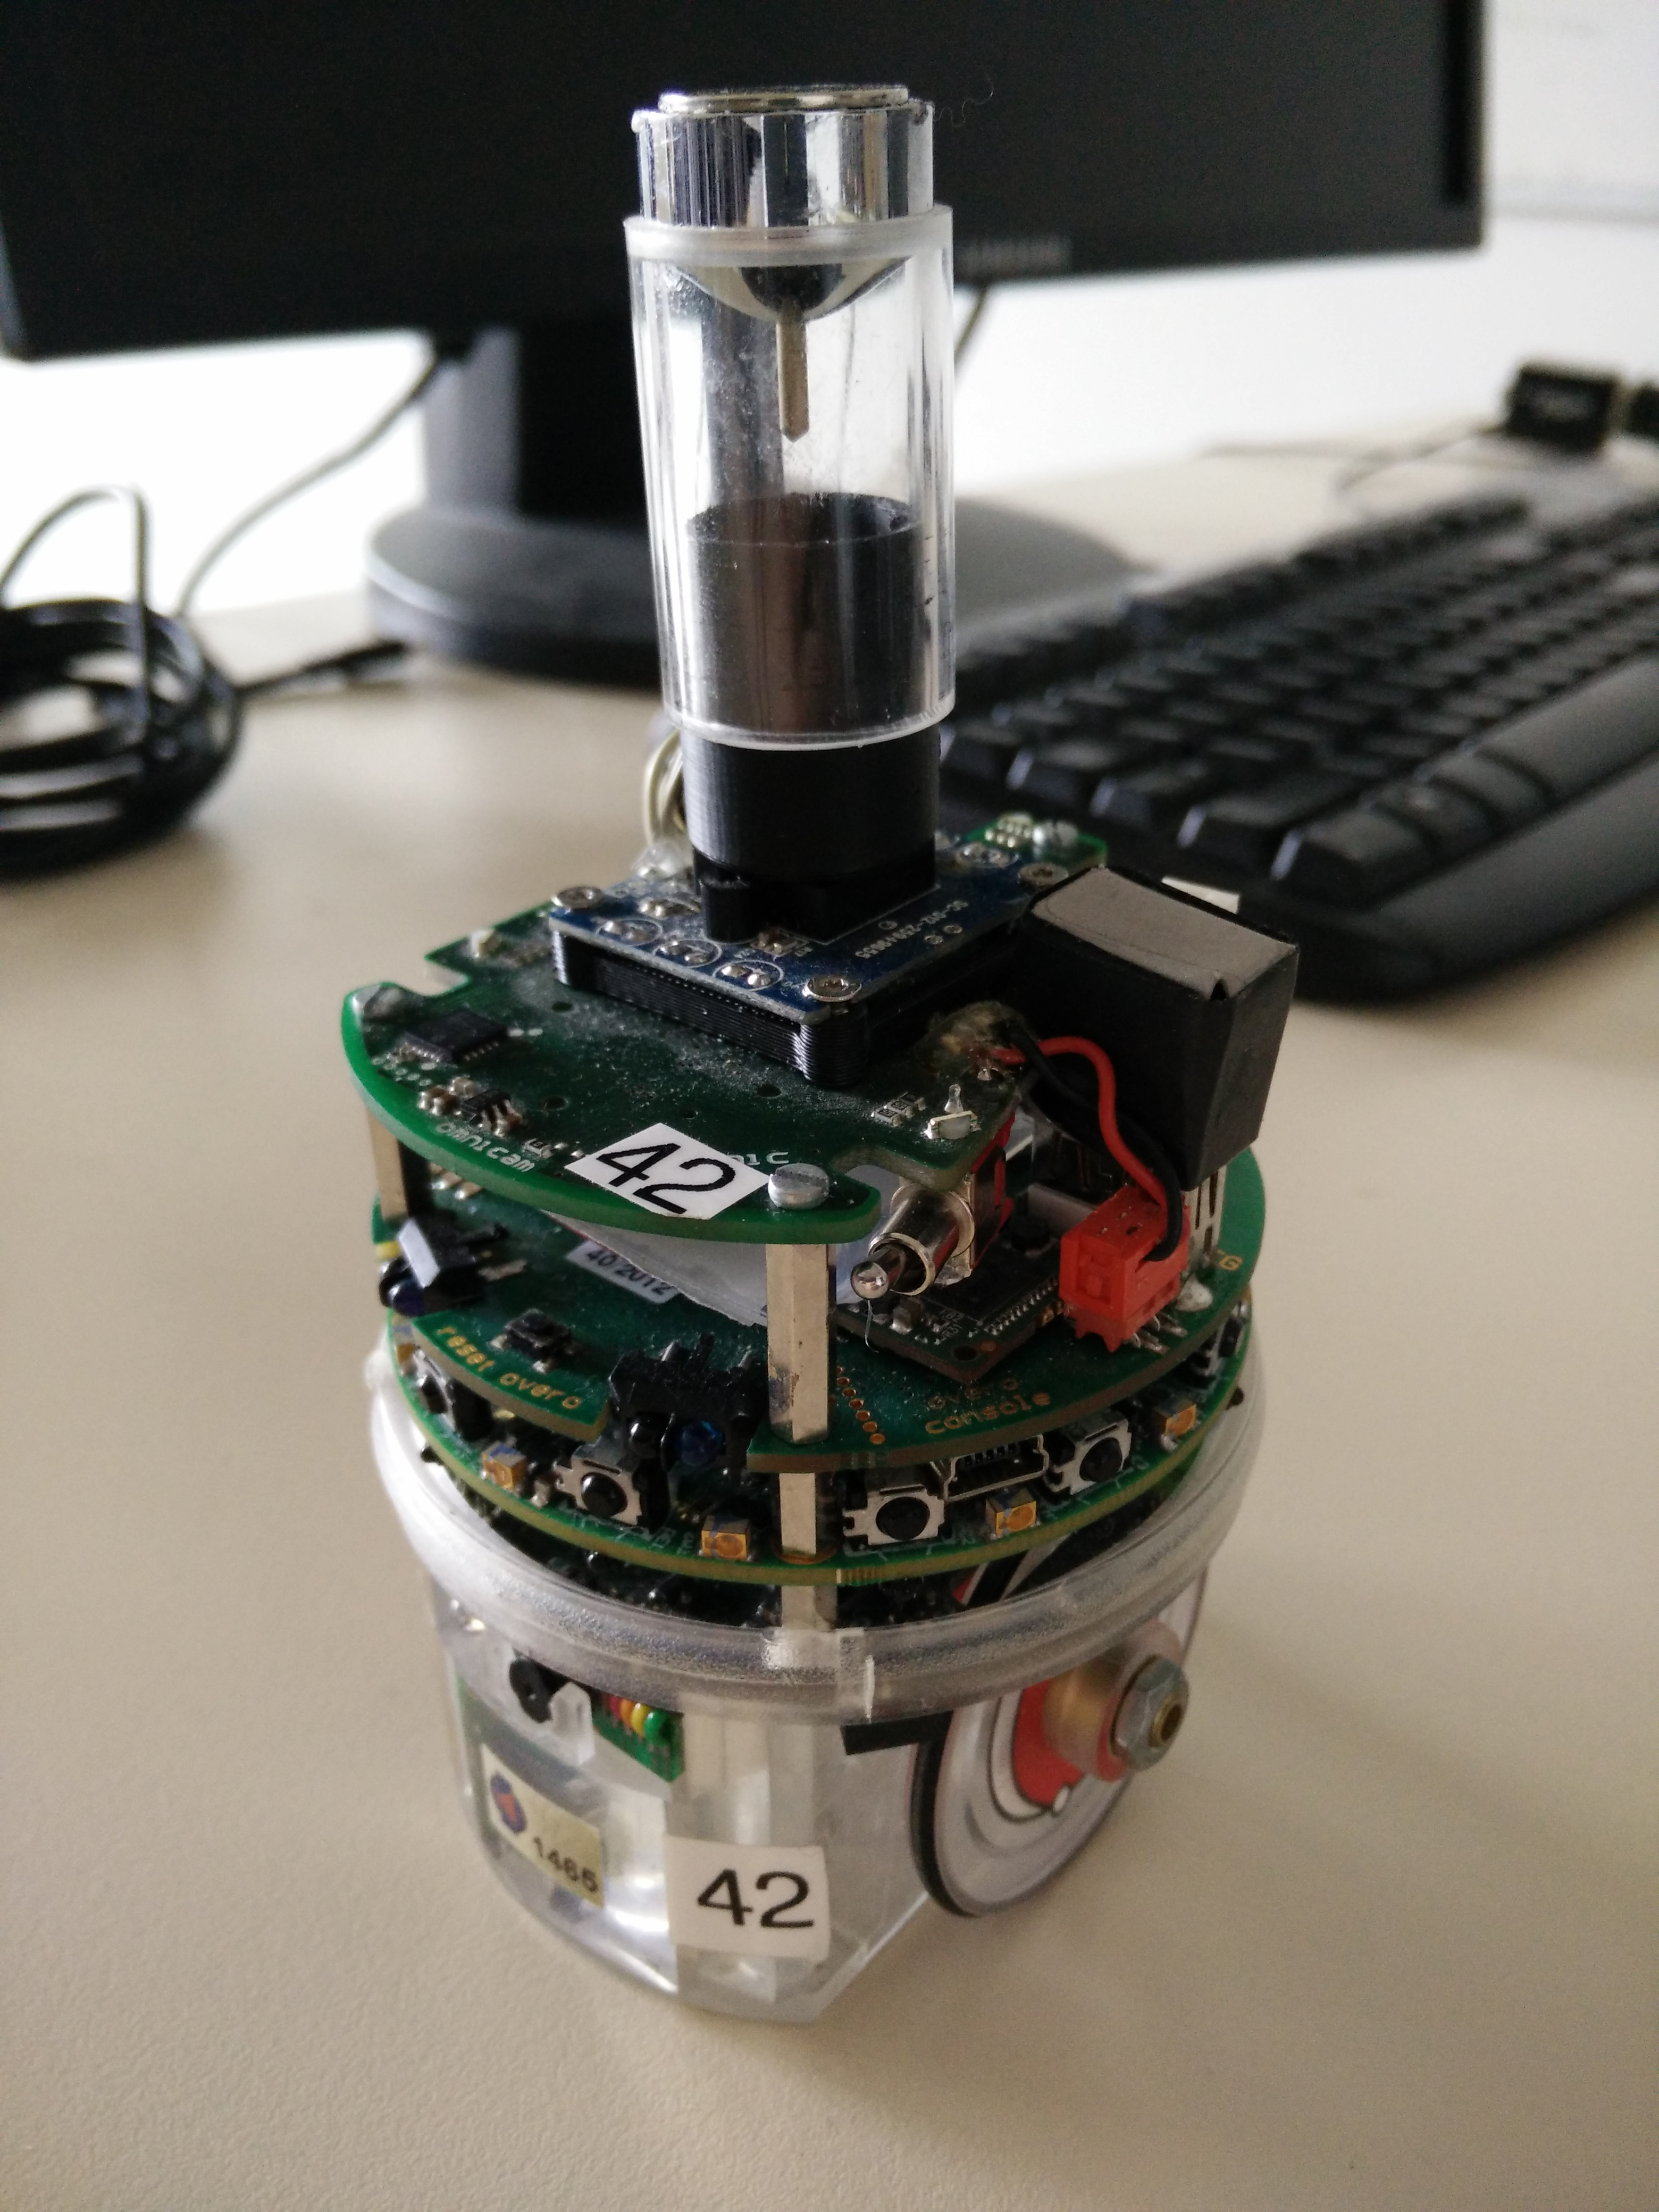
\includegraphics[width=3in]{../images/e-puck.jpg}
	\caption{The robotic platform we used: the E-puck.}
	\label{fig:e-puck}
\end{figure}

\begin{figure}[!t]
	\centering
	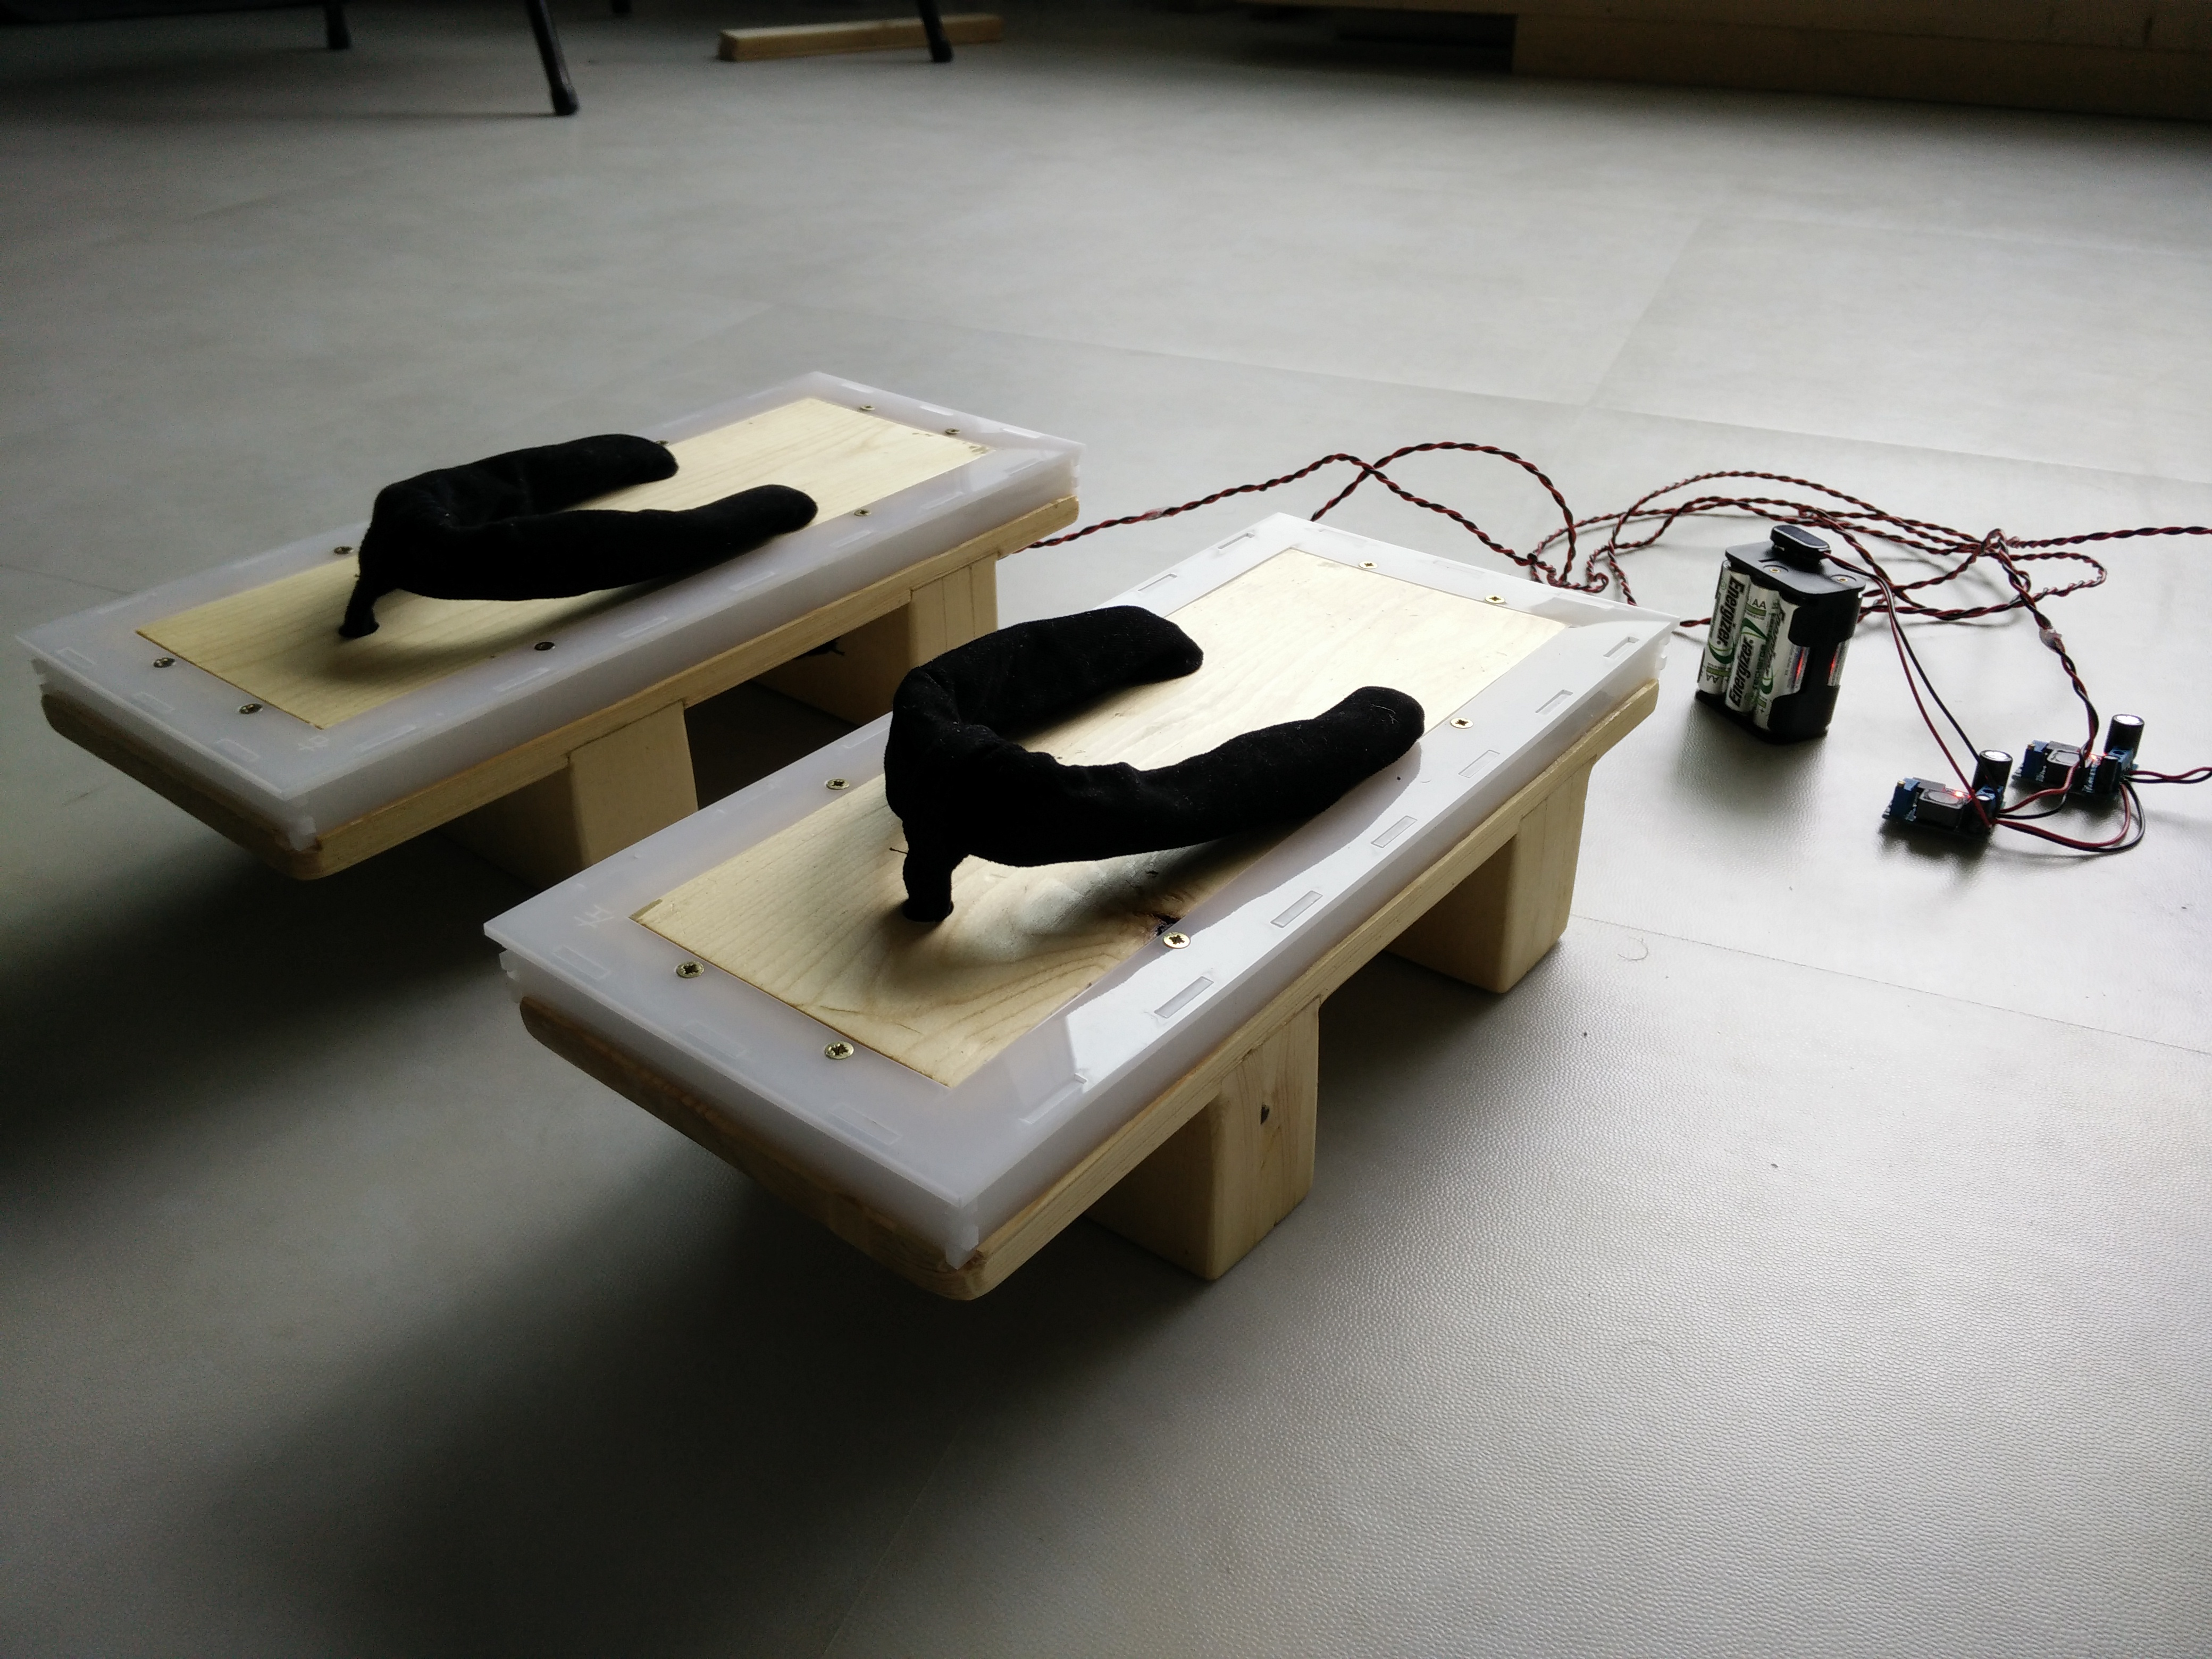
\includegraphics[width=3in]{../images/shoes2.jpg}
	\caption{The augmented shoes.}
	\label{fig:shoes}
\end{figure}

We conducted multiple experiments in simulations and with real robots to show that our solution addresses our problem. We characterised the system composed by the swarm of robots and the shoes by performing more tests: we tested the range of detection of the shoes to see how far away the robots could detect them. The maximum distance we obtained is sufficient for our purpose, but not for real applications. We also analysed the time needed by the robots to form a circle around the human from different starting positions. We obtained the best results for the starting configuration where all the robots are randomly placed in the arena. On the other hand we obtained longer delays for the configuration where all the robots are clustered near the shoes (this configuration is similar to a storage configuration). However, in all the cases, the robots surrounded the human. We ran an experiment with a human walking with the augmented shoes towards a virtual dangerous area. The robots in contact with the dangerous area correctly warned the human. Even though our solution satisfied our main problem (i.e., how to protect a human from going into dangerous areas), we believe that the current implementation of our solution has some limitations. These limitations could be investigated as future works.

%\subsection{Subsection Heading Here}
%Subsection text here.
%
%% needed in second column of first page if using \IEEEpubid
%%\IEEEpubidadjcol
%
%\subsubsection{Subsubsection Heading Here}
%Subsubsection text here.


% An example of a floating figure using the graphicx package.
% Note that \label must occur AFTER (or within) \caption.
% For figures, \caption should occur after the \includegraphics.
% Note that IEEEtran v1.7 and later has special internal code that
% is designed to preserve the operation of \label within \caption
% even when the captionsoff option is in effect. However, because
% of issues like this, it may be the safest practice to put all your
% \label just after \caption rather than within \caption{}.
%
% Reminder: the "draftcls" or "draftclsnofoot", not "draft", class
% option should be used if it is desired that the figures are to be
% displayed while in draft mode.
%
%\begin{figure}[!t]
%\centering
%\includegraphics[width=2.5in]{myfigure}
% where an .eps filename suffix will be assumed under latex, 
% and a .pdf suffix will be assumed for pdflatex; or what has been declared
% via \DeclareGraphicsExtensions.
%\caption{Simulation results for the network.}
%\label{fig_sim}
%\end{figure}

% Note that IEEE typically puts floats only at the top, even when this
% results in a large percentage of a column being occupied by floats.
% However, the Computer Society has been known to put floats at the bottom.


% An example of a double column floating figure using two subfigures.
% (The subfig.sty package must be loaded for this to work.)
% The subfigure \label commands are set within each subfloat command,
% and the \label for the overall figure must come after \caption.
% \hfil is used as a separator to get equal spacing.
% Watch out that the combined width of all the subfigures on a 
% line do not exceed the text width or a line break will occur.
%
%\begin{figure*}[!t]
%\centering
%\subfloat[Case I]{\includegraphics[width=2.5in]{box}%
%\label{fig_first_case}}
%\hfil
%\subfloat[Case II]{\includegraphics[width=2.5in]{box}%
%\label{fig_second_case}}
%\caption{Simulation results for the network.}
%\label{fig_sim}
%\end{figure*}
%
% Note that often IEEE papers with subfigures do not employ subfigure
% captions (using the optional argument to \subfloat[]), but instead will
% reference/describe all of them (a), (b), etc., within the main caption.
% Be aware that for subfig.sty to generate the (a), (b), etc., subfigure
% labels, the optional argument to \subfloat must be present. If a
% subcaption is not desired, just leave its contents blank,
% e.g., \subfloat[].


% An example of a floating table. Note that, for IEEE style tables, the
% \caption command should come BEFORE the table and, given that table
% captions serve much like titles, are usually capitalized except for words
% such as a, an, and, as, at, but, by, for, in, nor, of, on, or, the, to
% and up, which are usually not capitalized unless they are the first or
% last word of the caption. Table text will default to \footnotesize as
% IEEE normally uses this smaller font for tables.
% The \label must come after \caption as always.
%
%\begin{table}[!t]
%% increase table row spacing, adjust to taste
%\renewcommand{\arraystretch}{1.3}
% if using array.sty, it might be a good idea to tweak the value of
% \extrarowheight as needed to properly center the text within the cells
%\caption{An Example of a Table}
%\label{table_example}
%\centering
%% Some packages, such as MDW tools, offer better commands for making tables
%% than the plain LaTeX2e tabular which is used here.
%\begin{tabular}{|c||c|}
%\hline
%One & Two\\
%\hline
%Three & Four\\
%\hline
%\end{tabular}
%\end{table}


% Note that the IEEE does not put floats in the very first column
% - or typically anywhere on the first page for that matter. Also,
% in-text middle ("here") positioning is typically not used, but it
% is allowed and encouraged for Computer Society conferences (but
% not Computer Society journals). Most IEEE journals/conferences use
% top floats exclusively. 
% Note that, LaTeX2e, unlike IEEE journals/conferences, places
% footnotes above bottom floats. This can be corrected via the
% \fnbelowfloat command of the stfloats package.




%\section{Conclusion}
%The conclusion goes here.





% if have a single appendix:
%\appendix[Proof of the Zonklar Equations]
% or
%\appendix  % for no appendix heading
% do not use \section anymore after \appendix, only \section*
% is possibly needed

% use appendices with more than one appendix
% then use \section to start each appendix
% you must declare a \section before using any
% \subsection or using \label (\appendices by itself
% starts a section numbered zero.)
%


%\appendices
%\section{Proof of the First Zonklar Equation}
%Appendix one text goes here.
%
%% you can choose not to have a title for an appendix
%% if you want by leaving the argument blank
%\section{}
%Appendix two text goes here.
%
%
% use section* for acknowledgment
\ifCLASSOPTIONcompsoc
  % The Computer Society usually uses the plural form
  \section*{Acknowledgments}
\else
  % regular IEEE prefers the singular form
  \section*{Acknowledgment}
\fi


The author would like to thank Mauro Birattari, Ga\"{e}tan Podevijn, Andreagiovanni Reina, Anthony Antoun, Brian Delhaisse, Lorenzo Garattoni and the IRIDIA laboratory for their precious help and the hardware provided.


% Can use something like this to put references on a page
% by themselves when using endfloat and the captionsoff option.
\ifCLASSOPTIONcaptionsoff
  \newpage
\fi



% trigger a \newpage just before the given reference
% number - used to balance the columns on the last page
% adjust value as needed - may need to be readjusted if
% the document is modified later
%\IEEEtriggeratref{8}
% The "triggered" command can be changed if desired:
%\IEEEtriggercmd{\enlargethispage{-5in}}

% references section

% can use a bibliography generated by BibTeX as a .bbl file
% BibTeX documentation can be easily obtained at:
% http://www.ctan.org/tex-archive/biblio/bibtex/contrib/doc/
% The IEEEtran BibTeX style support page is at:
% http://www.michaelshell.org/tex/ieeetran/bibtex/
\bibliographystyle{IEEEtran}
% argument is your BibTeX string definitions and bibliography database(s)
%\bibliography{IEEEabrv,../bib/paper}
%
% <OR> manually copy in the resultant .bbl file
% set second argument of \begin to the number of references
% (used to reserve space for the reference number labels box)
%\begin{thebibliography}{1}
%
%\bibitem{IEEEhowto:kopka}
%H.~Kopka and P.~W. Daly, \emph{A Guide to \LaTeX}, 3rd~ed.\hskip 1em plus
%  0.5em minus 0.4em\relax Harlow, England: Addison-Wesley, 1999.
%
%\end{thebibliography}

\bibliography{thesis}

% biography section
% 
% If you have an EPS/PDF photo (graphicx package needed) extra braces are
% needed around the contents of the optional argument to biography to prevent
% the LaTeX parser from getting confused when it sees the complicated
% \includegraphics command within an optional argument. (You could create
% your own custom macro containing the \includegraphics command to make things
% simpler here.)
%\begin{IEEEbiography}[{\includegraphics[width=1in,height=1.25in,clip,keepaspectratio]{mshell}}]{Michael Shell}
% or if you just want to reserve a space for a photo:

%\begin{IEEEbiography}{Michael Shell}
%Biography text here.
%\end{IEEEbiography}

% if you will not have a photo at all:
\begin{IEEEbiographynophoto}{Mauro Birattari}
Promoter. \href{mailto:mbiro@ulb.ac.be}{mbiro@ulb.ac.be}
\end{IEEEbiographynophoto}

\begin{IEEEbiographynophoto}{Marco Dorigo}
Co-promoter. \href{mailto:mdorigo@ulb.ac.be}{mdorigo@ulb.ac.be}
\end{IEEEbiographynophoto}

\begin{IEEEbiographynophoto}{Ga\"{e}tan Podevijn}
Supervisor. \href{mailto:gpodevij@ulb.ac.be}{gpodevij@ulb.ac.be}
\end{IEEEbiographynophoto}

\begin{IEEEbiographynophoto}{Andreagiovanni Reina}
Supervisor. \href{mailto:areina@ulb.ac.be}{areina@ulb.ac.be}
\end{IEEEbiographynophoto}

\vfill

% insert where needed to balance the two columns on the last page with
% biographies
%\newpage

%\begin{IEEEbiographynophoto}{Jane Doe}
%Biography text here.
%\end{IEEEbiographynophoto}

% You can push biographies down or up by placing
% a \vfill before or after them. The appropriate
% use of \vfill depends on what kind of text is
% on the last page and whether or not the columns
% are being equalized.

%\vfill

% Can be used to pull up biographies so that the bottom of the last one
% is flush with the other column.
%\enlargethispage{-5in}



% that's all folks
\end{document}


